
% !TEX root = main.tex

\chapter{The basics of StabFem }


In this chapter we explain the basic functionalities of StabFem. We recommend that you study the basic example \keys{EXAMPLE\_Lshape.m}.

This directory contains three freefem programs and a demo matlab script doing solving the following problem :


\section{Simple problem : solution of heat equation in a L-shaped domain}

1. Solve the steady heat conduction equations on a L-shaped domain with constant volumic source term $P$ and homogeneous Dirichlet boiundary conditions :

$$ \nabla^2 T = P  \mbox {  for } {\bf x} \in \Omega ; \quad T = 0   \mbox {  for } {\bf x} \in \Gamma$$

2.  Solve the unsteady heat conduction equations on a L-shaped domain with zero source term $P$ and time-periodic Dirichlet boundary conditions :

$$ 
 \partial T_1/\partial t= \nabla^2 T_1  \mbox {  for } {\bf x} \in \Omega ; \quad T_1 = T_w e^{i \omega t}   \mbox {  for } {\bf x} \in \Gamma
$$



\section{Matlab script and results}

The programs are sufficiently short to be fully given in these pages. See figures \ref{SCRIPT_Lshape.m},  \ref{Lshape_Mesh.edp}, \ref{Lshape_Steady.edp}.  

The reader already familiar with FreeFm++ should not have any provblem in undersanding the programs. If not, we recommand that you study the FreeFem++ Manual (chapter "Learning by examples").

The results are given in figure \ref{Lshape_Figures}.



\begin{figure*}[t]
\small
\lstinputlisting{../EXAMPLE_Lshape/SCRIPT_Lshape.m}
 \normalsize
\caption{
Matlab program \keys{SCRIPT\_Lshape.m})}
\label{SCRIPT_Lshape.m}
\end{figure*}


\begin{figure*}[t]
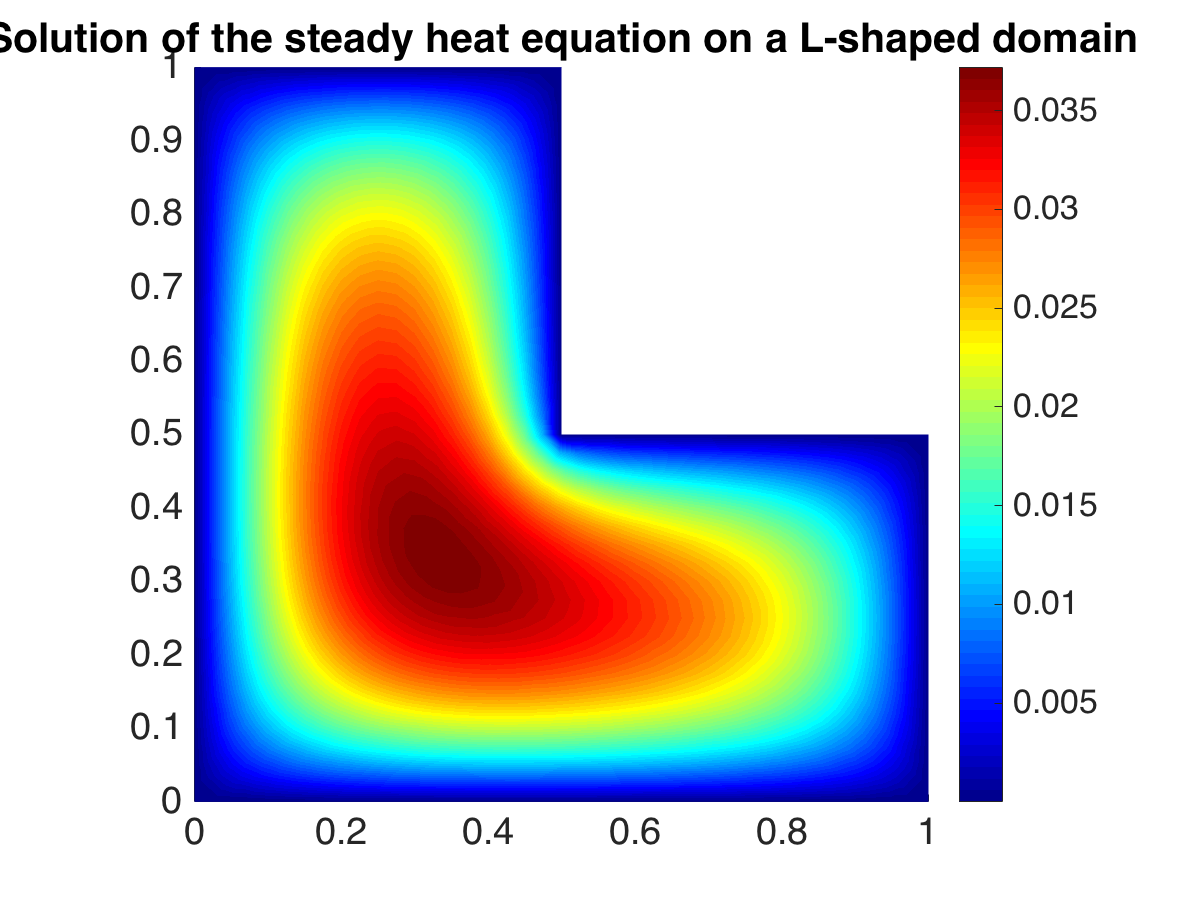
\includegraphics[width = .45 \linewidth]{../EXAMPLE_Lshape/FIGURES/Lshape_T0.png}
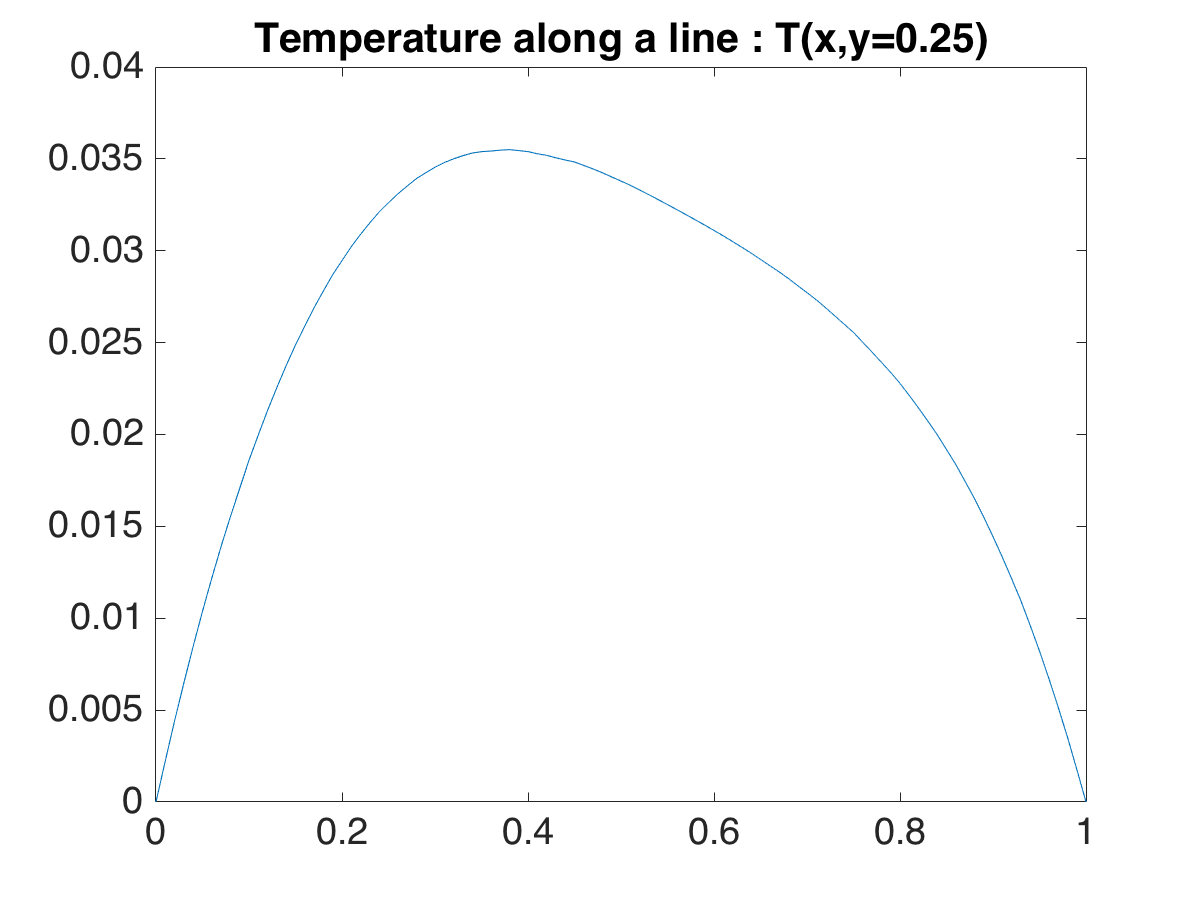
\includegraphics[width = .45 \linewidth]{../EXAMPLE_Lshape/FIGURES/Lshape_T0_Cut.png}
\caption{Solution for the steady hrat equation in a L-shape domain : $(a)$ Temperature field $T(x,y)$. 
$(b)$ Temperature $T(x,0.25)$ along a horizontal line. }
\label{Lshape_Figures}
\end{figure*}

\begin{figure*}[t]
\small
\lstinputlisting{../EXAMPLE_Lshape/Lshape_Mesh.edp}
 \normalsize
\caption{
FreeFem++ program \keys{Lshape\_Mesh.edp})}
\label{Lshape_Mesh.edp}
\end{figure*}


\begin{figure*}[t]
\small
\lstinputlisting{../EXAMPLE_Lshape/Lshape_Steady.edp}
\normalsize
\caption{
FreeFem++ program \keys{Lshape\_Steady.edp})}
\label{Lshape_Mesh.edp}
\end{figure*}


\clearpage

%%%%%%%%%%%%%%%%%%%%%%%%%%%%%%%%%%%%%%%%%%%%%%%
\section{How does it work ?}

\subsection{Analysis of the example}

Let us observe and explain the most important steps of the example matlab script \keys{SCRIPT\_Lshape.m}. 

\begin{itemize}
\item  The first step is {\bf creating and importing a mesh}. This is done by the function \keys{SF\_Mesh.m} invoked at line 7 of the script. 
Basically this function does the following operations :
\begin{enumerate}
\item Launch the FreeFem++ program \keys{Lshape\_Mesh.edp} with the {\em entry parameter} \footnote{Here and in the sequel, 
{\em entry parameter} means a value you will be invited to type on the keyboard if using directly FreeFem++ in the way you are used to. Just try !}
$Ndensity = 40$ (here corresponding to the mesh density).
\item Import the data produced by the FreeFem++ Macro {\sf SFWriteMesh} (more explanations in paragraph 3.3) 
\item Return the data as a Matlab {\em structure} object called {\sf ffmesh}
\end{enumerate}

Execution of this step leads to the following :
\lstinputlisting[linerange={1-15}]{Lshape_ExecutionExample.txt}

This structure objects has several fields which will serve for plotting data obtained on this mesh. See more in section 2.3.

\item The second step is {\bf launching a FreeFem program using this mesh and importing results}. 
This is done by the generic driver function \keys{SF\_Launch.m} invoked at line 12 of the script. 
Basically this function does the following operations :
\begin{enumerate}
\item Launch the FreeFem++ program \keys{Lshape\_Steady.edp}  (here with no {\em entry parameter}).
\item Import the data produced by the FreeFem++. By default the driver will look for a file called \keys{Data.ff2m}. 
This file is the one created by the FreeFem program in lines 14-22 of the Freefem program \ref{Lshape_Steady.edp}.

Looking inside the file \keys{Data.ff2m}, the header (i.e.  first four lines) is as follows :
\lstinputlisting[linerange={1-5}]{../EXAMPLE_Lshape/Data.ff2m}, 
meaning that this files contains a P1 mesh-organised field called 'T'.

\item Return the data as a matlab {\em structure} object called {\sf heatS}.
\end{enumerate}

Execution of this step leads to the following :
\lstinputlisting[linerange={17-24}]{Lshape_ExecutionExample.txt}

Where we can see that the structure has field called 'T' (containing the imported data)
 and a field called 'mesh'  which is actually the mesh object previously constructed and passed to the driver as a parameter as a field.


\item The third step which is important to explain ist {\bf importation of results previously generated by Freefem}. 
This is done by the generic driver function \keys{importFFdata.m} invoked at line 12 of the script. 

Here, besides the file Data.edp previously imported, our program has generated a second data file called \keys{Heat\_1Dcut.ff2m}.
%This file is the one created by the FreeFem program in lines 14-22 of the Freefem program \ref{Lshape_Steady.edp}.
The header of this file is as follows :
\lstinputlisting[linerange={1-5}]{../EXAMPLE_Lshape/Heat_1Dcut.ff2m}, 
meaning that this files contains two vectors of dimension 101 called X and T.


Execution of this step leads to the following :
\lstinputlisting[linerange={26-32}]{Lshape_ExecutionExample.txt}


Where we can see that the data is imported as a structure with two fields corresponding to the required data.

\end{itemize}

The \keys{importFFdata.m} functions is the core of the interface, and is actually internally called by the higher-levels drivers \keys{SF\_Mesh.m}  and \keys{SF\_Launch.m}.

 
%\caption{
%File \keys{Data.ff2m})}
%\label{Lshape_Data.ff2m}
%\end{figure*}

%File \keys{Heat\_1Dcut.ff2m}

%\lstinputlisting[linerange={1-5}]{../EXAMPLE_Lshape/Heat_1Dcut.ff2m}


%\lstinputlisting{../EXAMPLE_Lshape/ExecutionExample}

\subsection{Explanations of the \texttt{.ff2m} exchange format}


As can be seen in the previous short examples, the basis of the FreeFem/Matlab interface relies in the file exchange format \keys{.ff2m}
and the importation "wizard"  \keys{importFFdata.m} which reads these files.

Let us explain how such files are constituted. As we have observed, the header of a \keys{.ff2m} file has the following structure :

\lstinputlisting{Lshape_FormatExplanation.ff2m}.

The line 4 explains the nature of the data which is contained in the file.
There can be as many data objects as you want organised in the order of your choice. The recognized types are currently as follows :
\begin{description}
\item{ \bf P1}  for mesh-structured data stored as P1 finite-elements
\footnote{P2 data is not yet supported, the solution is to convert everything to P1 before exportation.}  
\item{\bf P1c}  for mesh-structured {\em complex} data stored as P1 finite-elements
\item{\bf real} for real scalars,
\item{\bf complex} for complex scalars,
\item{\bf real.N} for real vectors of dimension N not associated to a mesh,
\item{\bf complex.N} for complex vectors of dimension N not associated to a mesh,
\item{\bf P1s} for real data defined along a frontier of the mesh,
\item{\bf P1sc} for complex data defined along a frontier of the mesh.
\end{description}

\subsection{Explanations about the mesh }

to be continued...







